%!TEX root = ../template.tex
%%%%%%%%%%%%%%%%%%%%%%%%%%%%%%%%%%%%%%%%%%%%%%%%%%%%%%%%%%%%%%%%%%%%
%% chapter4.tex
%% NOVA thesis document file
%%
%% Chapter with lots of dummy text
%%%%%%%%%%%%%%%%%%%%%%%%%%%%%%%%%%%%%%%%%%%%%%%%%%%%%%%%%%%%%%%%%%%%

\typeout{NT FILE chapter4.tex}%

\chapter{Dimensional Inspection and Measurement Equipment}
\label{cha:lorem_ipsum}

This chapter introduces the equipment and methodology that can be used for dimensional inspection in engine component analysis. Keeping parts within the required tolerances is essential for ensuring performance and durability. A 3D scanner makes it possible to generate a digital model of the components, while a coordinate measuring machine (CMM) allows for precise measurement and comparison with nominal dimensions. These tools help improve the accuracy of the analysis and support potential optimization of the components at \gls{TAP} \gls{ME} Engine Shop.

The Engine Shop at \gls{TAP} \gls{ME} has a specialized Dimensional Inspection department responsible for verifying component dimensions in accordance with the manual, ensuring optimal engine performance and reliability.

\section{Available Measurement Equipment}
\label{sec:equipment}

To ensure precise measurements, the department relies on advanced equipment, such as the Creaform HandySCAN 3D scanner, which captures highly accurate digital models of components, and the Mitutoyo Euro-C 121210 coordinate measuring machine (CMM), which provides detailed dimensional and geometric analysis. By using these tools, the team can carry out thorough inspections, verify tolerances, and explore opportunities for improving component performance.

\subsection{Creaform HandySCAN 3D scanner}
\label{sec:scanner}

The HandySCAN 3D is a high-precision laser scanner developed by Creaform, designed for portable 3D scanning of objects with complex geometries. It uses laser triangulation to capture detailed 3D models with high accuracy and resolution.
It presents the following technical data: 
\begin{itemize}
    \item \textbf{Accuracy}: 0.025 mm (0.0009 in)
    \item \textbf{Volumetric Accuracy}: Up to 0.020 mm + 0.015 mm/m
    \item \textbf{Light Source}: 22–30 blue laser lines
    \item \textbf{Working Distance}: 200 to 750 mm
    \item \textbf{Recommended Part Size Range}: 0.05 – 4 m
    \item \textbf{Weight}: 0.94 kg
\end{itemize}

The HandySCAN 3D laser scanner is used in conjunction with VXelements, an integrated 3D software platform that allos real-time data acquisition, post-processing, and analysis.

During the development of this thesis, this equipment will enable the practice of reverse engineering. Using the HandySCAN 3D scanner, detailed physical data from the \gls{HPC} blades can be captured, and with the VXelements software, the point cloud is transformed into a 3D \gls{CAD} model. This model can then be imported into SolidWorks for further analysis and used to design the workpiece, which will be employed in the \gls{CMM} to securely hold the blades during measurement.

\subsection{Mitutoyo Euro-C 121210}
\label{sec:cmm}

The \gls{CMM} is a highly precise tool used to measure the geometry of parts and components. It works by using a probe that senses the physical contact with the object. While traditional CMMs rely on touch-trigger probes, there are other models that use laser or optical sensors to take measurements. The Mitutoyo Euro-C 121210 \gls{CMM} is controlled by a computer and operates within a three-dimensional coordinate system.

This particular CMM is equipped with a Renishaw Revo-2, providing it with five degrees of freedom (DoF). In addition to moving along the three main axes, the machine can adjust the probe’s angles, enabling it to measure even the most complex surfaces that would otherwise be difficult to reach. The machine setup includes a granite bed, probe, probe tree, arm, joystick, and specialized software, as shown in Figure~\ref{fig:cmm}.

Although four probes are available for use with the Renishaw Revo-2, only two are applicable to this project. Among them, the RSP2-3 is the sole probe that enables full five-degree-of-freedom operation. As illustrated in Figure~\ref{fig:dof}, the first three DoFs (X, Y, and Z) are controlled by the \gls{CMM} arm, while the remaining two ($\alpha$, $\beta$) are executed by the probe itself.

Each probe has distinct characteristics suited for different tasks, as detailed in Table~\ref{tab:probes}.


\begin{table}[ht]
    \caption{Renishaw probes available at TAP}
    \label{tab:probes}
    \centering
    \begin{tabular}{cccc}
    \toprule
    \textbf{Probe} & DoF & Scanning Capability & Sphere $\varnothing$ \\ \hline
    \textbf{RSP2-3} &  5 & 2D & 6mm \\ \hline
    \textbf{RSP3}  & 3 & 3D & 4mm \\ \hline
\end{tabular}
\end{table} 

\begin{figure}[H]
    \centering
    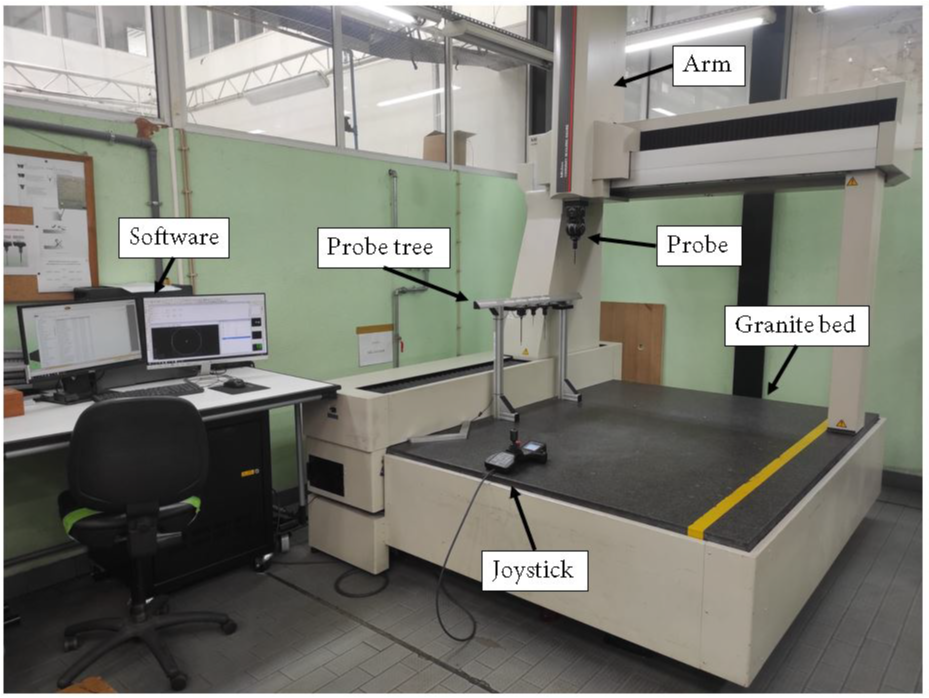
\includegraphics[width=0.8\textwidth]{cmm}
    \caption{Mitutoyo Euro-C 121210 Components \cite{Shi2023}}
    \label{fig:cmm}
\end{figure}

\begin{figure}[H]
    \centering
    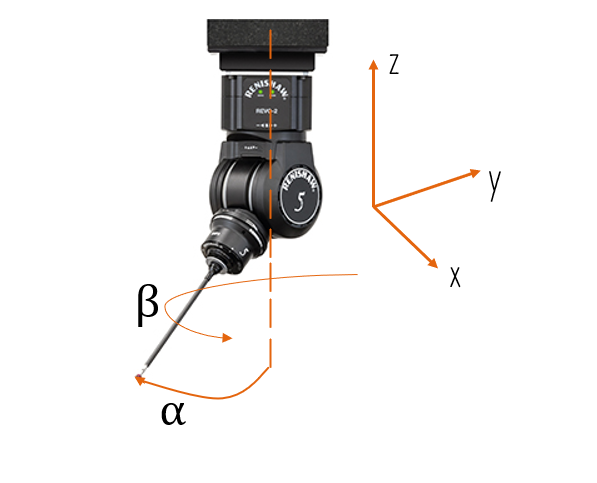
\includegraphics[width=0.4\textwidth]{dof}
    \caption{DOF of the Renishaw probe \cite{renishaw2025}}
    \label{fig:dof}
\end{figure}

The integration of the \gls{CMM} into this project plays a key role in ensuring that every high-pressure compressor rotor blade is measured quickly, accurately, and consistently. The development of a custom inspection program aims to enable the production team to measure entire sets of blades with minimal manual intervention, enhancing both efficiency and reliability.

Through the use of the \gls{CMM}, it is possible to automatically verify critical dimensions, such as \gls{CL}, \gls{LET}, \gls{TET}, and overall airfoil geometry. This ensures that each blade meets the required tolerances while eliminating inconsistencies associated with manual measurement methods. Additionally, this automation reduces the workload of operators, allowing them to focus on other essential tasks while the machine performs the measurements.

Another significant advantage of the \gls{CMM} is its ability to generate detailed inspection reports, facilitating the tracking of blade conditions over time. This capability extends beyond simple compliance verification, contributing to predictive maintenance strategies that enhance engine performance and reduce unexpected maintenance costs.

By incorporating this level of automation and precision into the inspection process, the proposed approach aims to streamline production, improve quality control, and establish a more efficient and standardized methodology for \gls{TAP}’s maintenance operations.

\section{TAP ME: Previous Theses on Dimensional Inspection}
\label{sec:before}

In the past, several master's theses have been developed in collaboration with \gls{TAP} \gls{ME}, contributing to the improvement of measurement and inspection processes for aircraft engine components. One of these studies was conducted by Farinha, E. \cite{Farinha2021}, focusing on the design of a fixture and the development of a measurement method for high-pressure compressor (HPC) rotor blades. This research continued the work initiated by Rendas, P. [13], who laid the foundation for the development of a fixture specifically designed for HPC rotor blade inspection.

Additionally, Baptista, F. \cite{rendas2021fixture} contributed to this field by developing a model that predicts the off-design performance of the CFM56-5B turbofan engine. More recently, Guerreiro, A. \cite{guerreiro} worked on the development of a process to measure the exit flow area of the low-pressure turbine (LPT) nozzles from the same engine model. His study focused on creating an automated program for Coordinate Measuring Machine (CMM) inspection, addressing a previously undeveloped process within \gls{TAP} \gls{ME}’s engine maintenance operations.

While previous studies have primarily focused on components of the CFM56-5B engine, this thesis aims to extend the dimensional inspection process to the HPC rotor blades of the LEAP-1A engine. One project involves developing an optimized CMM measurement program for assessing the blade chord to evaluate performance, utilizing data from the test bank. The second project focuses on measuring and controlling platform clearance to optimize the assembly process. These improvements, applied to both the LEAP and CFM engines, build on previous research, further advancing the continuous optimization of inspection methods to adapt to newer engine generations.


\chapter{Current Progress and Work Plan}
\label{cha:planeamento}

The analysis of the operation of the Maintenance and Engineering Unit included a demonstration of the component scanning process and a session on the functionality of the \gls{CMM}. Following this, the process through which blades go through maintenance was described in detail, as shown in Figure~\ref{fig:esquema}, outlining each step in the maintenance cycle.

Additionally, a collection of scrapped \gls{HPC} blades from a \gls{LEAP}-1A engine was carried out, involving the tracking of blades that had been discarded during previous maintenance activities. This collection enabled the scanning and dimensional comparison between a new and a worn blade, with the goal of analyzing the extent of blade degradation over time and understanding its potential impact on performance.

In parallel, work on test cell data analysis was initiated, aiming to develop a program to assess the impact of variations in sensor readings on the final engine \gls{EGT} measurement. This analysis seeks to identify key parameters that influence test cell results and to understand how performance evaluation is carried out. By gaining deeper insights into these factors, it will be possible to facilitate future analyses of the impact of blade chord length variations on engine performance.

\begin{figure}[H]
    \centering
    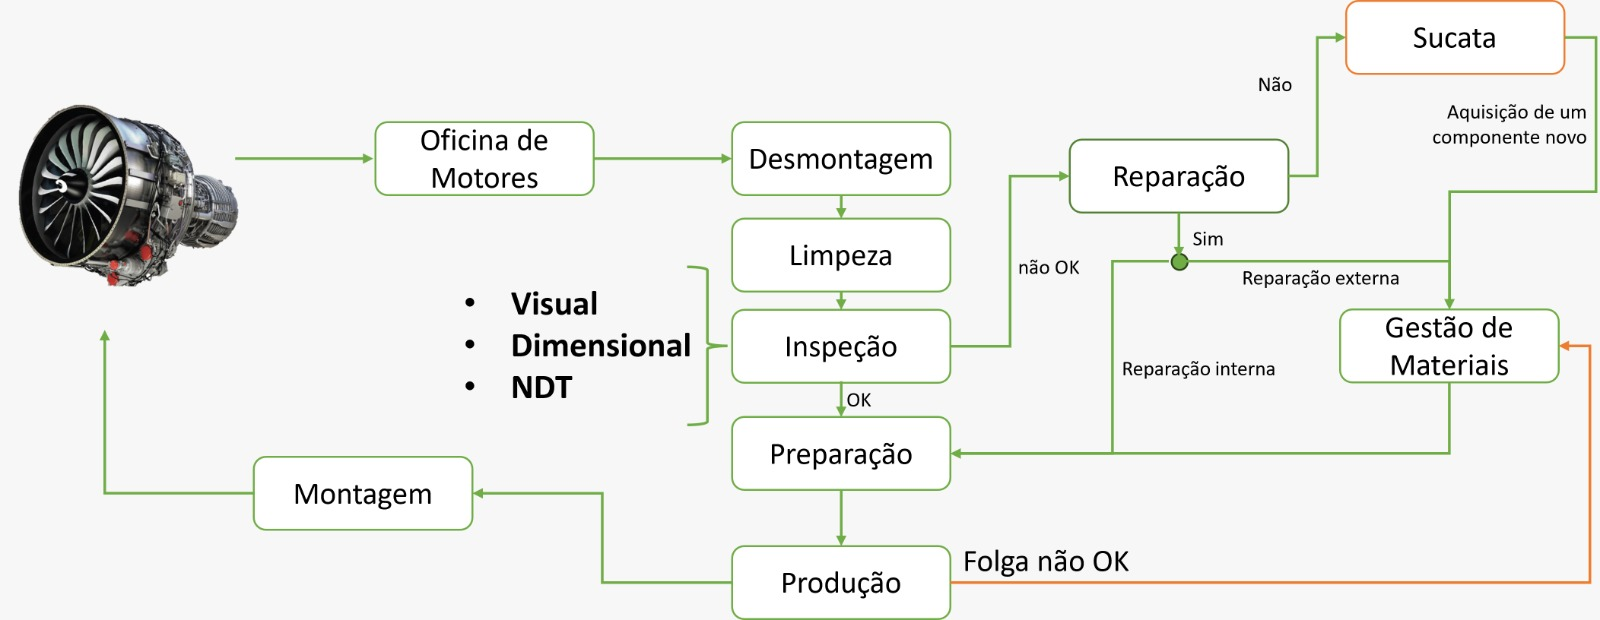
\includegraphics[width=0.8\textwidth]{esquema.jpeg}
    \caption{Process overview of blade maintenance cycle}
    \label{fig:esquema}
\end{figure}

\section{Work Plan}
\label{sec:plano}

To ensure a well-structured and efficient workflow, a provisional task plan has been created, as shown in Figure~\ref{fig:plan_prov}. The schedule will distribute key tasks over the coming months, allowing a balanced approach between research, development, and documentation. The initial phase focused on bibliographic research and drafting the dissertation introduction, providing a solid theoretical foundation. At the same time, work on scan processing and measurement tools will begin, setting the groundwork for later stages. Midway through the project, efforts will shift toward programming for chord measurement and analyzing test bench data—crucial steps for assessing engine performance. The final months will be dedicated to wrapping up the dissertation and completing the internship, ensuring all research components are properly integrated and documented. This structured approach is expected to help develop a project with practical value for the company while providing a highly enriching learning experience for the student.

\begin{figure}[H]
    \centering
    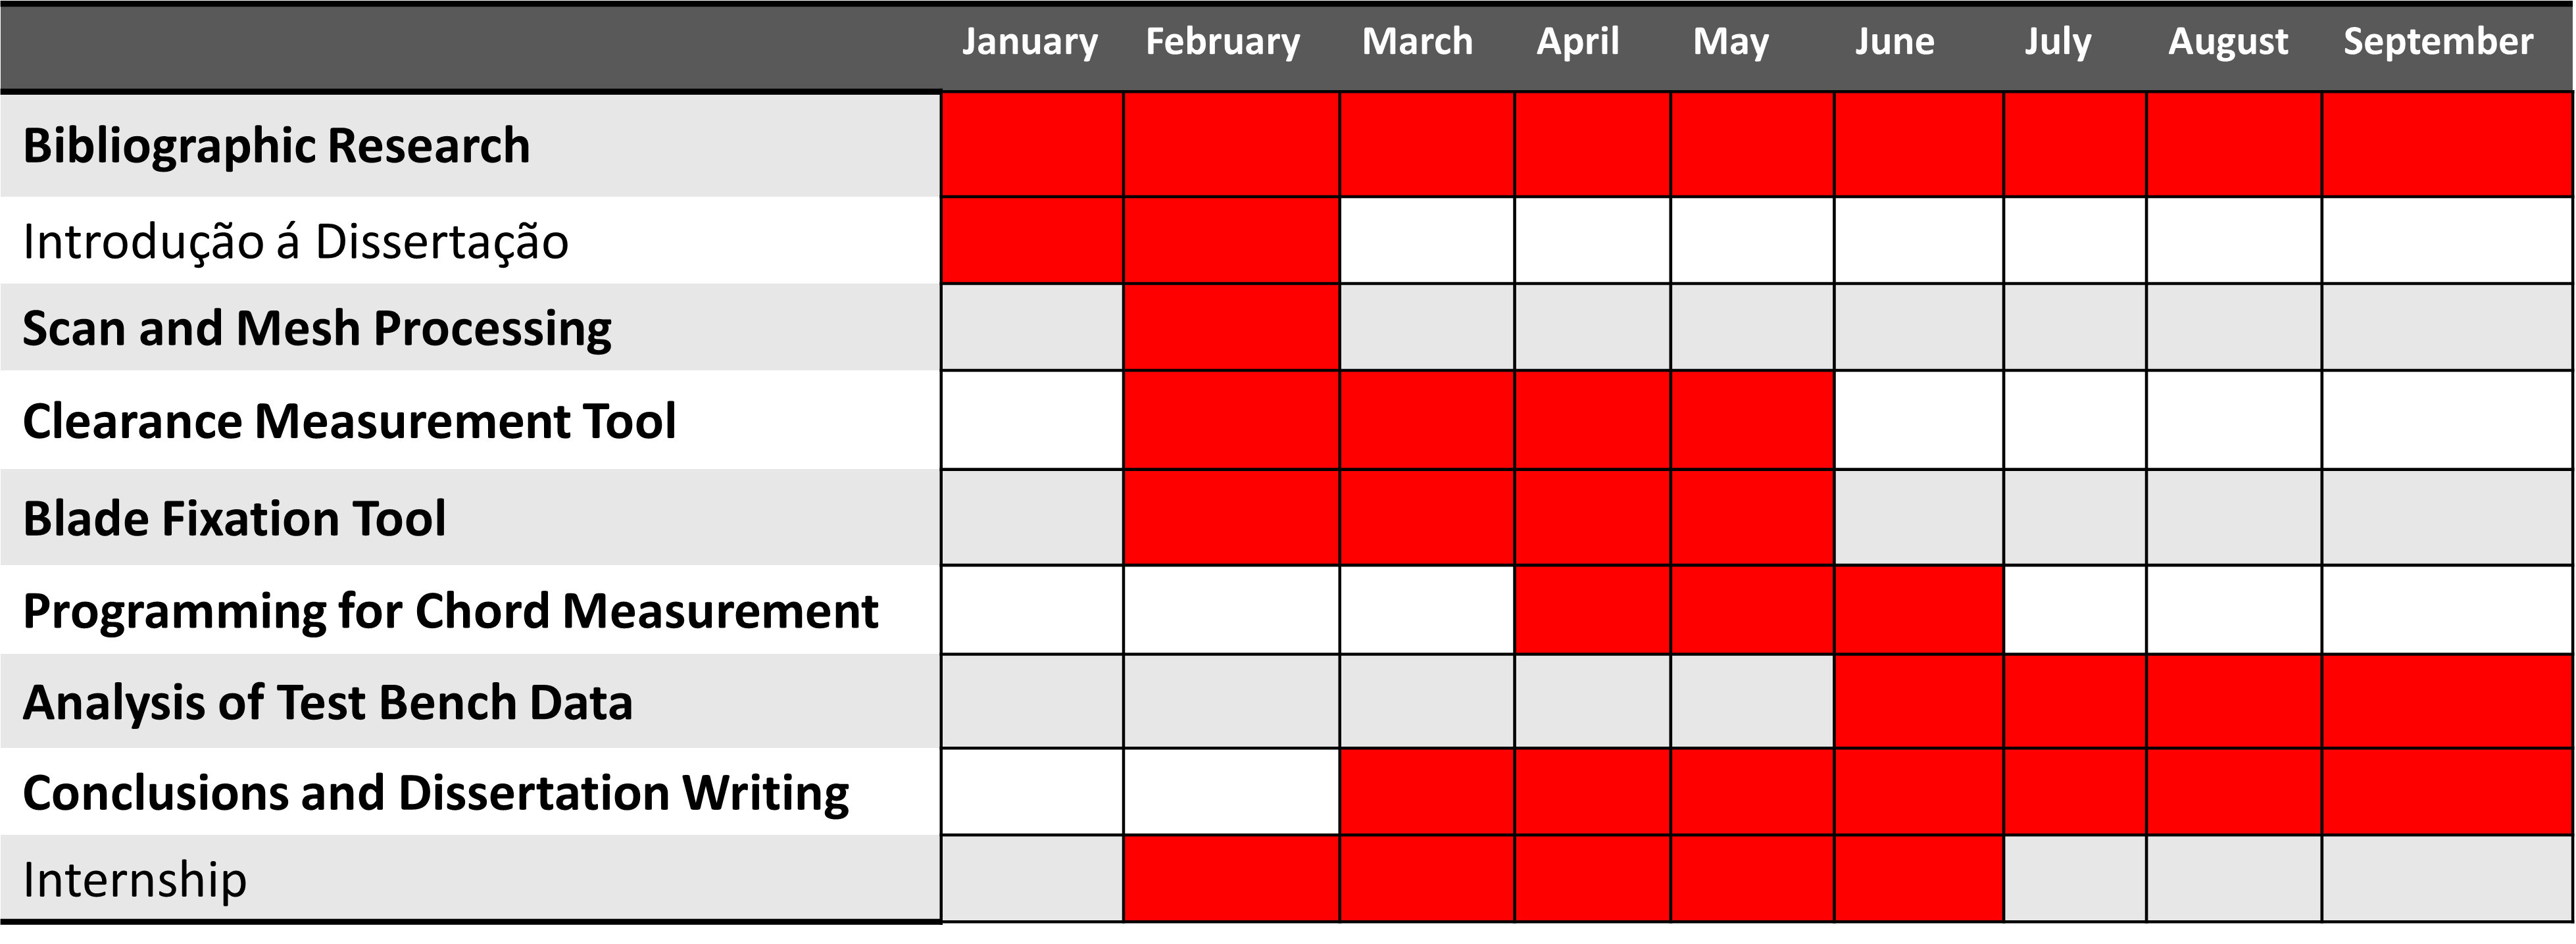
\includegraphics[width=0.8\textwidth]{plan_prov}
    \caption{Work Plan.}
    \label{fig:plan_prov}
\end{figure}


